
\section{Prueba de vuelo}

Se realizó una prueba de vuelo para comprobar el funcionamiento del controlador Delta 2.0 en un UAV de ala fija. Esta prueba se realizó en la Pista de Aeromodelismo Vuelo Libre, en Tenjo, Cundinamarca, Colombia. 

El controlador de vuelo fue instalado en el fuselaje de un avión tipo Protégé de Carl Goldberg, justo debajo de las alas. Esta ubicación estratégica permite un fácil acceso y brinda la protección adecuada para los componentes electrónicos durante el vuelo. (veasé \ref{fig:protege})

\begin{itemize}
    \item \textbf{Imagen Izquierda:} La imagen muestra la instalación del controlador de vuelo dentro del fuselaje del avión. Se puede ver que el controlador está firmemente sujeto justo debajo de las alas. Esta posición facilita la conexión con otros componentes del sistema de vuelo y asegura que el controlador permanezca estable durante el vuelo.
    
    \item \textbf{Imagen Derecha:} La imagen muestra el UAV-RAS Uniandes tipo Protégé completamente ensamblado y listo para volar. Se puede apreciar cómo el controlador de vuelo está integrado de manera discreta en el fuselaje, sin interferir con la aerodinámica del avión.
\end{itemize}


\begin{figure}[H]
    \centering
    \includegraphics[width=\textwidth]{Imagenes/Pruebas/UAV protegé.png}
    \caption{Instalación del Controlador de Vuelo Protégé}
    \label{fig:protege}
\end{figure}


\subsection{Metodología de la Prueba}

En esta prueba se tiene una comunicación bidireccional entre la tarjeta en base y la tarjeta en vuelo. La tarjeta en base es conectada mediante un cable tipo C de transmisión de datos a un ordenador que despliega la interfaz, tal como se muestra en la figura \ref{fig:diagrama_prueba_vuelo}.

Las pruebas que se llevaron a cabo se dividen en cinco categorías principales: Sensórica, Actuadores, GPS, Comunicación, Almacenamiento de Datos e Interfaz. Las pruebas se llevaron a cabo en tres fases: en tierra, durante el montaje en el UAV y en vuelo.\\


En la categoría de sensórica, las lecturas del giroscopio (Yaw, Pitch y Roll) fueron precisas en todas las fases, obteniendo una calificación del 100\%. Sin embargo, en las pruebas del barómetro se presentaron picos abruptos en las lecturas de presión atmosférica y altura durante el vuelo, lo que no fue consistente con la información de vuelo. Estos cambios abruptos en la recepción de datos resultaron en una calificación del 50\%.\\

En cuanto a los actuadores, estos funcionaron perfectamente al usar el receptor FlySky. Estos mostraron un funcionamiento óptimo tanto en tierra como en vuelo, obteniendo una calificación del 100\%. Durante las pruebas en el montaje del UAV se presentaron delays en las señales del controlador y los servos, lo que resultaría en una afectación en las dinámicas del UAV. Por otro lado, debido a condiciones climáticas no se pudo realizar una prueba de vuelo con el controlador Delta 2.0 por lo que durante el vuelo con el FlySky se posicionó el controlador de vuelo en el interior del UAV pero sin conectar los servos del UAV a este.\\

En la categoría de GPS, la calibración y recepción de datos fueron correctas en tierra y durante el montaje en el UAV. Sin embargo, durante el vuelo, el tiempo de actualización del GPS no fue lo suficientemente rápido, lo que llevó a pérdidas de conexión con el satélite y resultó en una calificación del 70\%. Este problema causó saltos abruptos en la localización del UAV.\\

La Comunicación bidireccional entre la estación en tierra y el UAV fue efectiva en tierra, pero durante el vuelo se presentaron corrupciones de paquetes que afectaron la transmisión y recepción de datos. Esto resultó en calificaciones del 85\% y 30\% para la transmisión de datos del giroscopio y el barómetro, respectivamente. Además, hubo una gran pérdida de datos respecto a los datos transmitidos por la tarjeta en vuelo.\\

En la categoría de Almacenamiento de Datos, tanto la estación en tierra como el controlador de vuelo fueron capaces de almacenar datos correctamente en tierra. Sin embargo, durante el vuelo, hubo pérdidas ocasionales de datos, resultando en una calificación del 70\% para el controlador de vuelo. Este problema fue causado por la frecuencia de datos transmitidos y la capacidad de almacenamiento del sistema.\\

Finalmente, en la categoría de Interfaz, el despliegue y la visualización de datos fueron correctos en tierra. Sin embargo, durante el vuelo, se observaron delays y corrupción de datos en la tarjeta de vuelo, resultando en una calificación del 50\%. La tarjeta de la estación en tierra funcionó adecuadamente, pero la tarjeta de vuelo mostró problemas significativos.\\
\begin{figure}[H]
    \centering
    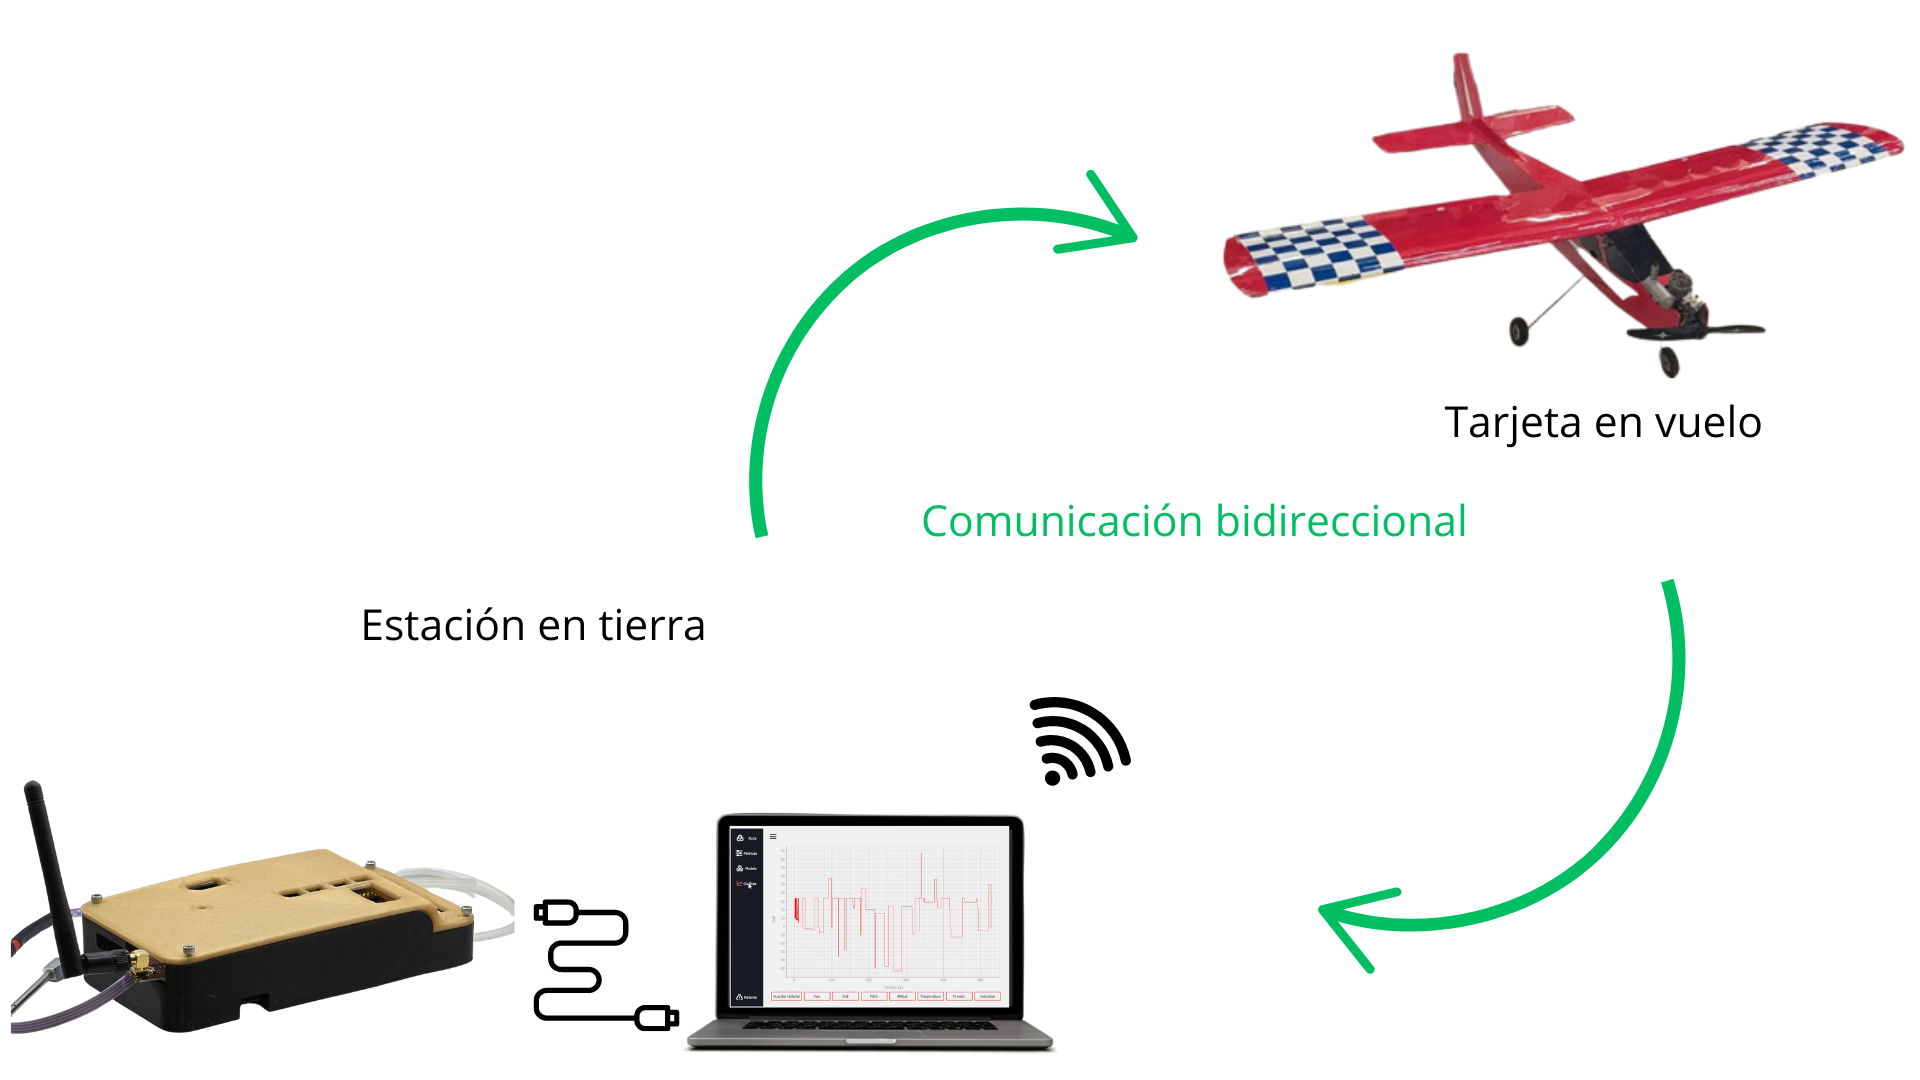
\includegraphics[width=12  cm]{Imagenes/Pruebas/Esquematico.png}
    \caption{Diagrama de la prueba de vuelo}
    \label{fig:diagrama_prueba_vuelo}
\end{figure}


\clearpage
\subsection{Matriz de Rendimiento de la Prueba de vuelo}
A continuación se muestra la matriz de rendimiento de la prueba de vuelo\ref{fig:matriz_prueba_vuelo}:

\begin{figure}[H]
    \centering
    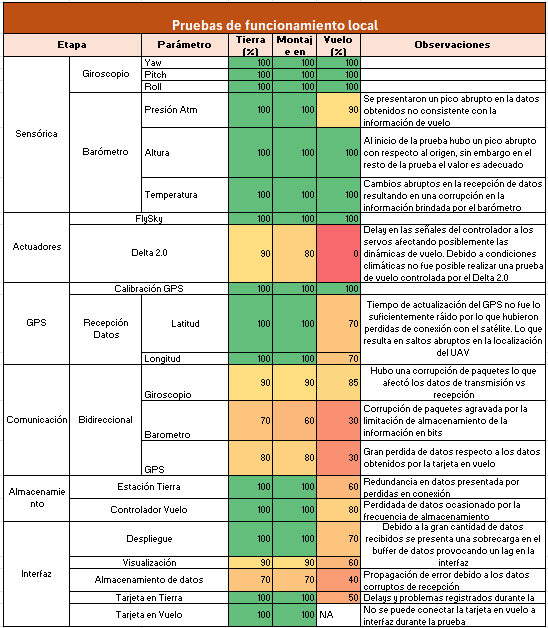
\includegraphics[width=\textwidth]{Imagenes/Pruebas/matriz_prueba_vuelo_local.png}
    \caption{Matriz de evaluación para prueba de vuelo}
    \label{fig:matriz_prueba_vuelo}
\end{figure}

El desempeño general de las pruebas evidencia un comportamiento sólido en tierra y durante el montaje en el UAV. Por otro lado, se evidencian algunas dificultades notables durante las pruebas de vuelo, especialmente en las áreas de comunicación bidireccional, almacenamiento de datos y la interfaz de usuario. Estas áreas requieren una revisión y optimización para asegurar un rendimiento óptimo en condiciones de vuelo.

A continuación se muestra el rendimiento general de la prueba de vuelo\ref{fig:resumen_prueba_vuelo}:

\begin{figure}[H]
    \centering
    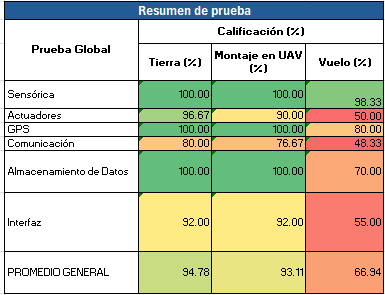
\includegraphics[width=10cm]{Imagenes/Pruebas/resumen_prueba_vuelo_local.png}
    \caption{Matriz de evaluación para prueba de vuelo}
    \label{fig:resumen_prueba_vuelo}
\end{figure}